\documentclass[11pt,a4paper]{article}

% ---------------------------------------------------------------------------
% Packages
% ---------------------------------------------------------------------------
\usepackage[margin=1in]{geometry}
\usepackage{amsmath,amssymb,amsthm}
\usepackage{booktabs}
\usepackage{hyperref}
\usepackage{listings}
\usepackage{xcolor}
\usepackage{tikz}
\usetikzlibrary{arrows.meta,positioning,shapes.geometric,fit,calc}
\usepackage{enumitem}
\usepackage{microtype}
\usepackage{url}
\usepackage{fancyhdr}
\usepackage{titlesec}

% ---------------------------------------------------------------------------
% Hyperref
% ---------------------------------------------------------------------------
\hypersetup{
  colorlinks=true,
  linkcolor=blue!60!black,
  citecolor=blue!60!black,
  urlcolor=blue!60!black,
  pdftitle={promptconf Theory},
  pdfauthor={promptconf},
  pdfsubject={Filesystem-native prompt versioning theory}
}

% ---------------------------------------------------------------------------
% Listings
% ---------------------------------------------------------------------------
\lstdefinestyle{promptconf}{
  basicstyle=\ttfamily\small,
  breaklines=true,
  frame=single,
  rulecolor=\color{black!30},
  backgroundcolor=\color{gray!5},
  columns=fullflexible,
  keepspaces=true,
  showstringspaces=false,
  aboveskip=0.8em,
  belowskip=0.8em,
  xleftmargin=0.5em,
  xrightmargin=0.5em
}
\lstset{style=promptconf}

% ---------------------------------------------------------------------------
% Page style
% ---------------------------------------------------------------------------
\pagestyle{fancy}
\fancyhf{}
\fancyhead[L]{\small\texttt{promptconf} Theory}
\fancyhead[R]{\small v0.3.0}
\fancyfoot[C]{\thepage}
\renewcommand{\headrulewidth}{0.4pt}

\titleformat{\section}{\large\bfseries}{\thesection}{1em}{}
\titleformat{\subsection}{\normalsize\bfseries}{\thesubsection}{1em}{}

% ---------------------------------------------------------------------------
% Macros
% ---------------------------------------------------------------------------
\newcommand{\pc}{\texttt{promptconf}}
\newcommand{\code}[1]{\texttt{#1}}
\newcommand{\botperp}{\bot}

\begin{document}

% ===========================================================================
\title{\pc{} --- Theory}
\author{promptconf v0.3.0}
\date{}
\maketitle

\begin{abstract}
This document formalizes \pc{} v0.3.0: filesystem-native prompt versioning,
pluggable backends, the version-resolution algebra (\code{latest}, tags, lock
pins), dual template engines, compile caching, embedding search, deterministic
A/B assignment, the closed-loop performance ledger, and lint-as-static-analysis.
All claims track the public API in \code{promptconf.loader}, \code{backends},
\code{cache}, \code{ledger}, \code{vcs}, \code{template}, \code{ab}, and
\code{lint}.
\end{abstract}

\tableofcontents
\newpage

% ===========================================================================
\section{Problem statement}
% ===========================================================================

Prompts are software artifacts: edited often, A/B tested, and easy to lose
track of when inlined as string literals. \pc{} provides an offline,
git-friendly store:
\begin{equation}
  \mathrm{load}(n,\, v,\, x;\; R,\, e,\, B) \;\longrightarrow\; \text{string}
\end{equation}
where $n$ is the prompt name, $v$ a version selector, $x$ template variables,
$R$ the root, $e \in \{\texttt{format},\texttt{jinja}\}$ the engine, and $B$ an
optional \code{PromptBackend}.

Root resolution precedence: explicit \code{root} $\rightarrow$ env
\code{PROMPTCONF\_ROOT} $\rightarrow$ \code{./prompts}. Bound API:
\code{PromptStore(root=\ldots, backend=\ldots)}.

% ===========================================================================
\section{Store geometry}
\label{sec:store}
% ===========================================================================

\begin{lstlisting}
R / n /  {v}.{txt,md,prompt}
\end{lstlisting}

\begin{itemize}[leftmargin=*]
  \item Prompt \textbf{names} $=$ immediate subdirectories of $R$
        (skip \texttt{.}--prefixed dirs).
  \item Version \textbf{stems} are file stems under $R/n/$.
  \item Extension priority when stems collide:
        \texttt{.txt} $\succ$ \texttt{.md} $\succ$ \texttt{.prompt}.
  \item Optional YAML frontmatter (\texttt{---} \ldots\ \texttt{---}) is
        stripped before render; \code{compile\_prompt} exposes metadata $+$ body.
  \item Empty / path-like names and empty versions $\rightarrow$
        \code{ValidationError}.
  \item Files larger than \code{MAX\_PROMPT\_BYTES} (1\,MiB, overridable via
        \code{max\_bytes=}) $\rightarrow$ \code{PromptSizeError}.
\end{itemize}

Version stem classes:
\begin{enumerate}[leftmargin=*]
  \item Numeric releases matching \verb|^v(\d+)$|
        (case-insensitive): \code{v1}, \code{v2}, \code{v10}.
  \item Alias file stem \code{latest} (optional).
  \item Arbitrary other stems (listed alphabetically between numerics and
        \code{latest}).
\end{enumerate}

% ===========================================================================
\section{Version resolution algebra}
% ===========================================================================

Define $V(n)$ as the set of available stems for prompt $n$.

\subsection{Explicit version}

\begin{equation}
  \mathrm{resolve}(n,\, v) \;=\;
  \begin{cases}
    \mathrm{path}(v) & \text{if } v \in V(n) \\
    \botperp         & \text{otherwise (raises \texttt{PromptNotFoundError})}
  \end{cases}
\end{equation}

\subsection{\texttt{version="latest"} (floating alias)}

\begin{equation}
  \mathrm{resolve}(n,\, \texttt{latest}) \;=\;
  \begin{cases}
    \mathrm{path}(\texttt{latest})
      & \text{if } \texttt{latest} \in V(n) \\[0.4em]
    \mathrm{path}(v_{k^{*}})
      & \text{if } k^{*} = \max\{k : v_k \in V(n)\} \\[0.4em]
    \botperp
      & \text{otherwise}
  \end{cases}
\end{equation}

An explicit \code{latest.*} file \textbf{wins} over the highest numeric
\code{vN}. This is intentional: \code{latest} is an alias, not
``max semver.''

\subsection{Tags (named pointers)}

\code{tag(name, version, tag\_name)} writes
\code{\{root\}/.promptconf/tags.json}:
\begin{equation}
  \mathrm{tags}[\textit{tag\_name}] \;=\; \{\textit{name}: n,\;
  \textit{version}: v\}
\end{equation}
\code{resolve\_tag(tag\_name)} returns that record. Tags are \textbf{not}
auto-applied inside \code{load()}; callers resolve then
\code{load(name, version=\ldots)}. Validation ensures the target version exists
before writing.

\subsection{Lock file (\texttt{freeze})}

\code{freeze(root=\ldots)} writes \code{\{root\}/prompt.lock.json} mapping each
prompt name $\rightarrow$ a pin:
\begin{enumerate}[leftmargin=*]
  \item Prefer stem \texttt{"latest"} if present in $V(n)$,
  \item Else highest numeric $vN$,
  \item Else last listed version.
\end{enumerate}

Each pin is touch-resolved via \code{load(\ldots, raw=True)} so broken pins fail
at freeze time. The lock is a \textbf{reproducibility artifact} for CI and
deploys; \code{load()} itself still takes an explicit \code{version=} (or
\code{"latest"}) --- use lock pins as the version argument at call sites or in
wrappers.

\begin{figure}[htbp]
  \centering
  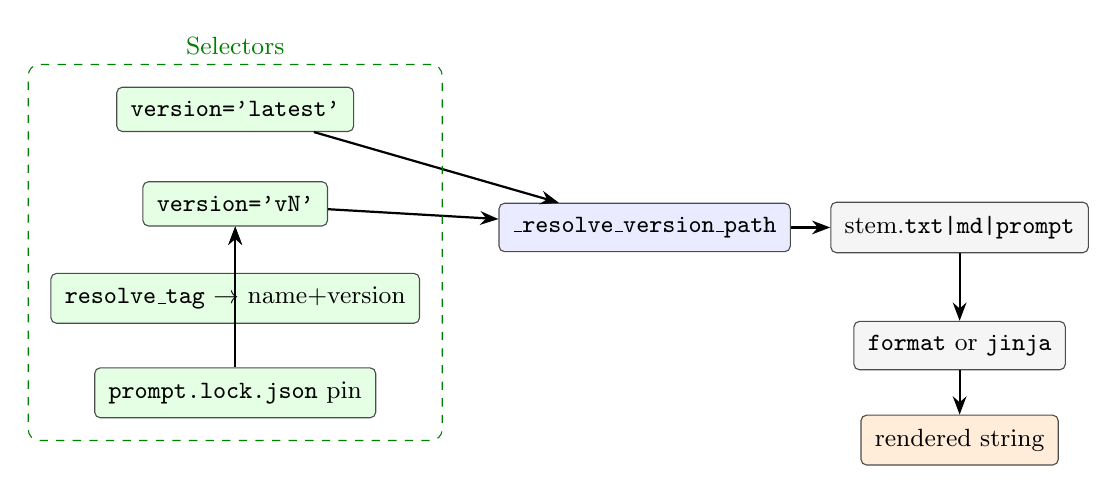
\begin{tikzpicture}[
    font=\small,
    box/.style={
      draw=black!70, rounded corners=2pt,
      align=center, inner sep=5pt,
      minimum height=1.6em
    },
    hub/.style={box, fill=blue!8},
    leaf/.style={box, fill=gray!8},
    arr/.style={-{Stealth}, thick}
  ]
    % Selectors
    \node[box, fill=green!10] (L) at (0,3) {\texttt{version='latest'}};
    \node[box, fill=green!10] (E) at (0,1.8) {\texttt{version='vN'}};
    \node[box, fill=green!10] (T) at (0,0.6)
      {\texttt{resolve\_tag} $\to$ name+version};
    \node[box, fill=green!10] (K) at (0,-0.6)
      {\texttt{prompt.lock.json} pin};

    \node[hub] (R) at (5.2,1.5) {\texttt{\_resolve\_version\_path}};
    \node[leaf] (F) at (9.2,1.5) {stem.\texttt{txt|md|prompt}};
    \node[leaf] (Eng) at (9.2,0) {\texttt{format} or \texttt{jinja}};
    \node[leaf, fill=orange!15] (Out) at (9.2,-1.2) {rendered string};

    \draw[arr] (L) -- (R);
    \draw[arr] (E) -- (R);
    \draw[arr] (T) -- (E);
    \draw[arr] (K) -- (E);
    \draw[arr] (R) -- (F);
    \draw[arr] (F) -- (Eng);
    \draw[arr] (Eng) -- (Out);

    \node[draw=green!50!black, dashed, rounded corners=4pt,
          fit=(L)(E)(T)(K), inner sep=8pt,
          label={[green!50!black]above:Selectors}] {};
  \end{tikzpicture}
  \caption{Version selectors funnel into path resolution, then template
    rendering. Tags and lock pins resolve externally to a concrete
    \texttt{version=} before \texttt{load}.}
  \label{fig:version-flow}
\end{figure}

\subsection{Listing order}

Numeric $v_k$ ascending $\rightarrow$ other non-\code{latest} stems alpha
$\rightarrow$ \code{latest} last. Used by \code{list\_versions} and error
messages.

% ===========================================================================
\section{Pluggable backends}
% ===========================================================================

\code{PromptBackend} protocol:

\begin{table}[htbp]
  \centering
  \begin{tabular}{@{}ll@{}}
    \toprule
    \textbf{Method} & \textbf{Role} \\
    \midrule
    \code{list\_prompts()}
      & Sorted names \\
    \code{list\_versions(name)}
      & Sorted stems \\
    \code{read(name, version)}
      & Raw file text (incl.\ frontmatter) \\
    \code{write(name, version, content)}
      & Optional; read-only backends may omit / error \\
    \bottomrule
  \end{tabular}
  \caption{\texttt{PromptBackend} protocol methods.}
  \label{tab:backend-protocol}
\end{table}

\paragraph{FilesystemBackend.}
Default; wraps the geometry in Section~\ref{sec:store}.

\paragraph{GitStoreBackend.}
Treat a local git path (or clone URL $+$ \code{cache\_dir}) as prompt root;
\code{read} from working tree; optional \code{commit} / \code{auto\_commit}.
Missing \code{git} CLI $\rightarrow$ \code{BackendUnavailableError}
(stdlib \code{subprocess}; \code{[git]} extra documents the dependency).

\code{load(\ldots, backend=B)} and \code{PromptStore(\ldots, backend=B)} are
additive. When \code{backend} is omitted, \code{load} uses the filesystem path
directly; \code{PromptStore} defaults to \code{FilesystemBackend(root)}.

% ===========================================================================
\section{Template engines}
\label{sec:templates}
% ===========================================================================

\subsection{\texttt{engine="format"} (default)}

Substitution via \code{str.format\_map} / \code{string.Formatter}:
\begin{equation}
  T(x) \;=\; \mathrm{format}(T_0,\, x)
\end{equation}

\begin{table}[htbp]
  \centering
  \begin{tabular}{@{}lp{0.62\textwidth}@{}}
    \toprule
    \textbf{Mode} & \textbf{Behavior} \\
    \midrule
    \code{strict=True}
      & Missing root keys $\rightarrow$ \code{PromptFormatError} \\
    \code{strict=False}
      & Missing keys left as literal \texttt{\{key\}} \\
    \code{raw=True}
      & Skip formatting; return body after frontmatter strip \\
    \bottomrule
  \end{tabular}
  \caption{Format-engine modes.}
  \label{tab:format-modes}
\end{table}

Root keys are the field names before \texttt{.}~/~\texttt{[} indexing.
Fail-closed strict mode prevents silent quality regressions from incomplete
instantiation.

\subsection{\texttt{engine="jinja"} (optional \texttt{[jinja]} extra)}

Rendering uses \code{jinja2.sandbox.SandboxedEnvironment} with
\code{PromptIncludeLoader} rooted at $R$:
\begin{itemize}[leftmargin=*]
  \item Context variables: \texttt{\{\{ var \}\}}, control:
        \texttt{\{\% if \%\}}, macros, etc.
  \item Includes / extends resolve under the prompt root.
  \item \code{StrictUndefined} when \code{strict=True}; soft undefined
        preserves \texttt{\{\{ name \}\}} when not strict.
  \item Unsafe attributes (\texttt{\_\_*\_\_}, \code{mro}, frame/code attrs,
        etc.) blocked via custom \code{is\_safe\_attribute}.
  \item \code{SecurityError} / syntax / missing includes surface as
        \code{PromptFormatError} or \code{PromptNotFoundError}.
\end{itemize}

\code{compile\_prompt} dry-runs parse validation without rendering (Jinja parse
or \code{Formatter().parse} for format engine).

\subsection{Compile cache}
\label{sec:cache}

\code{CompileCache(dir)} stores rendered strings under:
\begin{equation}
  k \;=\; \mathrm{SHA256}\!\bigl(
    \mathrm{canonical}(
      \textit{content},\, e,\, x_{\mathrm{sorted}},\, n,\, v
    )
  \bigr)
\end{equation}

\code{load(\ldots, use\_cache=True)} / \code{load\_cached(\ldots)} hit the cache
when $k$ matches. Content edits change the hash $\rightarrow$ automatic
invalidation (mtime alone is insufficient; bytes are authoritative). Default
cache dir: \code{\{root\}/.promptconf/cache}.

\subsection{Usage logging}

When \code{log=True}, appends JSONL under
\code{\{root\}/.promptconf/usage.jsonl} with \textbf{keys only} (never values)
--- reduces PII/secret leakage into the audit trail. \code{log(name)} (VCS
helper) filters that file by prompt name.

% ===========================================================================
\section{A/B hashing}
\label{sec:ab}
% ===========================================================================

\code{ABRouter(experiments, root=\ldots, seed=\ldots)} holds per-prompt weight
maps $\{v_i \mapsto w_i\}$ normalized to $\sum_i w_i = 1$.

\subsection{Deterministic assignment}

When \code{user\_id} is provided:
\begin{equation}
  b \;=\;
  \frac{\mathrm{int}_{16}\!\bigl(\mathrm{SHA256}(n{:}u)[:8]\bigr)}
       {2^{32}-1}
  \;\in\; [0,\,1)
\end{equation}
Then pick the first variant whose cumulative weight exceeds $b$ (last variant
is the residual). Sticky assignment: same $(n,\, u)$ always maps to the same
variant.

\subsection{Random assignment}

Without \code{user\_id}, draw $b \sim U[0,1)$ from an optional seeded
\code{random.Random}.

\code{choose} may log an \code{ab\_assignment} usage event; \code{load}
chooses then calls \code{promptconf.loader.load} for that version.

% ===========================================================================
\section{Closed-loop performance ledger}
\label{sec:ledger}
% ===========================================================================

\textbf{Differentiator.} Pins, tags, and A/B logs describe \emph{what ran}. The
ledger answers \emph{which prompt wins in production}.

Outcomes append to \code{\{root\}/.promptconf/outcomes.jsonl}:
\begin{equation}
  o_t \;=\; (n,\, v,\, m_k,\, m,\, u,\, \ldots)
\end{equation}
where $m_k$ defaults to \texttt{"reward"} and $m \in \mathbb{R}$ is an external
metric (task success, thumbs-up, latency inverse, \ldots).

\subsection{Aggregation}

\begin{equation}
  \mathrm{best\_version}(n;\, m_k,\, s_{\min}) \;=\;
  \operatorname*{argmax}_{v\,:\, |O_{n,v,m_k}| \,\ge\, s_{\min}}
  \mathrm{mean}(O_{n,v,m_k})
\end{equation}
Ties break by larger sample count, then version label. Returns $\emptyset$ when
no version meets $s_{\min}$.

\subsection{Recommend}

\begin{equation}
  \mathrm{recommend}(n,\, u) \;=\;
  \begin{cases}
    \mathrm{best\_version}(n)
      & \text{if defined} \\[0.3em]
    \mathrm{ABRouter.choose}(n,\, u)
      & \text{otherwise}
  \end{cases}
\end{equation}

This closes the loop: ship weighted variants $\rightarrow$ ingest outcomes
$\rightarrow$ promote winners without a cloud prompt hub.

Public surface: \code{record\_outcome}, \code{best\_version},
\code{recommend}, and bound helper
\code{PerformanceLedger(root=\ldots, router=\ldots)}. Outcomes live at
\code{\{root\}/.promptconf/outcomes.jsonl} (separate from
\code{usage.jsonl}).

\begin{figure}[htbp]
  \centering
  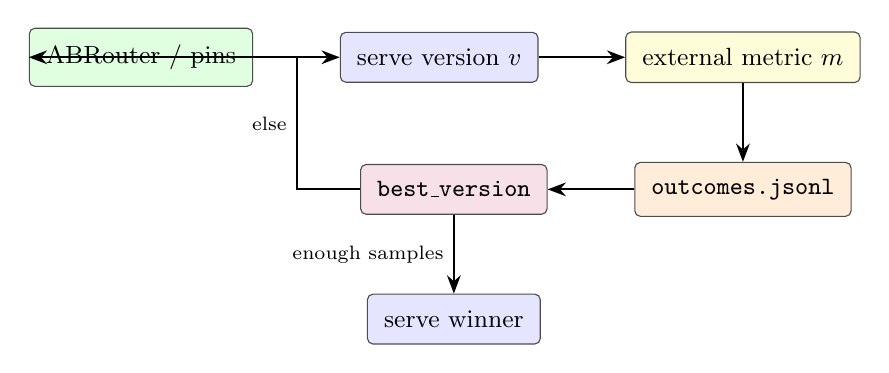
\begin{tikzpicture}[
    font=\small,
    box/.style={
      draw=black!70, rounded corners=2pt,
      align=center, inner sep=6pt,
      minimum height=1.8em
    },
    arr/.style={-{Stealth}, thick}
  ]
    \node[box, fill=green!12] (AB) {ABRouter / pins};
    \node[box, fill=blue!10, right=1.1cm of AB] (Serve) {serve version $v$};
    \node[box, fill=yellow!15, right=1.1cm of Serve] (Metric)
      {external metric $m$};
    \node[box, fill=orange!15, below=1.0cm of Metric] (Ledger)
      {\texttt{outcomes.jsonl}};
    \node[box, fill=purple!12, left=1.1cm of Ledger] (Best)
      {\texttt{best\_version}};
    \node[box, fill=blue!10, below=1.0cm of Best] (Serve2)
      {serve winner};

    \draw[arr] (AB) -- (Serve);
    \draw[arr] (Serve) -- (Metric);
    \draw[arr] (Metric) -- (Ledger);
    \draw[arr] (Ledger) -- (Best);
    \draw[arr] (Best) -- node[left, font=\scriptsize]{enough samples} (Serve2);
    \draw[arr] (Best.west) -- ++(-0.8,0) |- node[pos=0.25, left, font=\scriptsize]{else} (AB.west);
  \end{tikzpicture}
  \caption{Closed-loop ledger: A/B cold-start, metric ingest, winner promotion.}
  \label{fig:ledger-loop}
\end{figure}

% ===========================================================================
\section{Search: keyword vs semantic}
% ===========================================================================

\begin{itemize}[leftmargin=*]
  \item \code{search(query)} --- substring / regex over bodies;
        \code{SearchHit.score} denser/earlier matches.
  \item \code{semantic\_search(query, top\_k=\ldots)} --- embed query $+$
        bodies; rank by cosine similarity; same \code{SearchHit} shape with
        cosine \code{score}.
        \begin{itemize}
          \item Default embedder: \code{HashEmbedder} (deterministic
                bag-of-words hashing; offline/tests).
          \item Production: \code{OpenAIEmbedder} behind
                \code{[embeddings]}.
        \end{itemize}
\end{itemize}

Keyword \code{search()} is unchanged.

% ===========================================================================
\section{Lint as static analysis}
% ===========================================================================

Prompt lint is \textbf{static}: it inspects text without calling an LLM.
\code{LintRules} / \code{lint\_prompt} / \code{lint\_all} emit
\code{LintIssue} records (\code{rule}, \code{message}, \code{severity},
location).

\begin{table}[htbp]
  \centering
  \begin{tabular}{@{}lp{0.62\textwidth}@{}}
    \toprule
    \textbf{Rule} & \textbf{Idea} \\
    \midrule
    \code{max\_chars}
      & Length budget (error) \\
    \code{banned\_phrases}
      & Case-insensitive substring denylist (error) \\
    \code{require\_placeholders}
      & Must contain \texttt{\{name\}} format fields (error) \\
    \code{no\_trailing\_whitespace}
      & Line hygiene (warning) \\
    \code{json\_mode\_hint}
      & Regex detect JSON-output language: warn /
        \code{require} / \code{forbid} \\
    \bottomrule
  \end{tabular}
  \caption{Static lint rules.}
  \label{tab:lint-rules}
\end{table}

This is analogous to a linter AST pass: cheap, deterministic, CI-friendly.
Schema validation (\code{validate\_vars} / \code{load\_validated}) is a related
static check over declared variable contracts, separate from prose lint rules.

% ===========================================================================
\section{Diff, CLI, and companions}
% ===========================================================================

Conceptual companions (same package):
\begin{itemize}[leftmargin=*]
  \item \code{diff\_versions} --- textual diff across versions for review.
  \item CLI: \code{diff} / \code{tag} / \code{freeze} / \code{log} / lint-
        oriented workflows.
\end{itemize}

These do not change resolution algebra; they operationalize it for humans and
CI.

% ===========================================================================
\section{Design invariants}
% ===========================================================================

\begin{enumerate}[leftmargin=*]
  \item \textbf{Filesystem (or backend) is the registry} --- Git distributes;
        no cloud hub required.
  \item \textbf{\texttt{latest} is an alias, not $\max(vN)$ when a latest file
        exists.}
  \item \textbf{Tags and locks are pointers} --- resolve externally, then load
        by concrete version.
  \item \textbf{Strict formatting fails closed} by default.
  \item \textbf{Jinja is sandboxed} --- treat templates as untrusted when
        variables or includes are attacker-influenced.
  \item \textbf{Usage logs never store variable values.}
  \item \textbf{Ledger promotes winners from production metrics} --- A/B is
        the cold-start fallback.
  \item \textbf{Backends fail loud} when unavailable
        (\code{BackendUnavailableError}).
  \item \textbf{Oversized prompts fail loud}
        (\code{PromptSizeError} / \code{MAX\_PROMPT\_BYTES}).
  \item \textbf{Invalid names/versions fail loud}
        (\code{ValidationError}, also a \code{ValueError}).
\end{enumerate}

% ===========================================================================
\section{Mapping to source}
% ===========================================================================

\begin{table}[htbp]
  \centering
  \begin{tabular}{@{}lp{0.52\textwidth}@{}}
    \toprule
    \textbf{Concept} & \textbf{Module} \\
    \midrule
    Root, load, resolve, compile, \code{MAX\_PROMPT\_BYTES}
      & \code{promptconf.loader} \\
    Bound store
      & \code{promptconf.store.PromptStore} \\
    Backends
      & \code{promptconf.backends}
        (\code{FilesystemBackend}, \code{GitStoreBackend}) \\
    Compile cache
      & \code{promptconf.cache}
        (\code{CompileCache}, \code{load\_cached}) \\
    Performance ledger
      & \code{promptconf.ledger}
        (\code{record\_outcome}, \code{best\_version}, \code{recommend}) \\
    Semantic search
      & \code{promptconf.semantic\_search} \\
    Exceptions
      & \code{promptconf.exceptions}
        (\code{ValidationError}, \code{BackendUnavailableError},
         \code{PromptSizeError}, \ldots) \\
    Tags, freeze, usage log read
      & \code{promptconf.vcs} \\
    Jinja sandbox
      & \code{promptconf.template} \\
    Includes loader
      & \code{promptconf.includes} \\
    A/B router
      & \code{promptconf.ab} \\
    Lint
      & \code{promptconf.lint} \\
    Frontmatter
      & \code{promptconf.meta} \\
    Schema validation
      & \code{promptconf.schema} \\
    \bottomrule
  \end{tabular}
  \caption{Concept-to-module mapping.}
  \label{tab:source-map}
\end{table}

% ===========================================================================
\section{References}
% ===========================================================================

\begin{enumerate}[leftmargin=*,label={[\arabic*]}]
  \item Liu, P., et al.\ (2021).
        \emph{Pre-train, Prompt, and Predict.}
        \url{https://arxiv.org/abs/2107.13586}
  \item Khattab, O., et al.\ (2023).
        \emph{DSPy.}
        \url{https://arxiv.org/abs/2310.03714}
  \item Schulhoff, S., et al.\ (2024).
        \emph{The Prompt Report.}
        \url{https://arxiv.org/abs/2406.06608}
  \item Jinja2 SandboxedEnvironment documentation (template isolation).
  \item Python \code{string.Formatter} (format-engine field parsing).
  \item OpenAI Embeddings API (optional semantic search).
\end{enumerate}

\end{document}
